\documentclass[10pt,landscape]{article}
\usepackage{multicol}
\usepackage{calc}
\usepackage{ifthen}
\usepackage[landscape]{geometry}
\usepackage{hyperref}
\usepackage{amssymb}
\usepackage{amsmath}
\usepackage{graphicx}
\usepackage[utf8]{inputenc}
\usepackage{fullpage}
\usepackage[upright]{fourier}
\usepackage{tkz-graph}
\usepackage{alltt}
\usetikzlibrary{arrows}

% To make this come out properly in landscape mode, do one of the following
% 1.
%  pdflatex latexsheet.tex
%
% 2.
%  latex latexsheet.tex
%  dvips -P pdf  -t landscape latexsheet.dvi
%  ps2pdf latexsheet.ps


% If you're reading this, be prepared for confusion.  Making this was
% a learning experience for me, and it shows.  Much of the placement
% was hacked in; if you make it better, let me know...


% 2008-04
% Changed page margin code to use the geometry package. Also added code for
% conditional page margins, depending on paper size. Thanks to Uwe Ziegenhagen
% for the suggestions.

% 2006-08
% Made changes based on suggestions from Gene Cooperman. <gene at ccs.neu.edu>


% To Do:
% \listoffigures \listoftables
% \setcounter{secnumdepth}{0}


% This sets page margins to .5 inch if using letter paper, and to 1cm
% if using A4 paper. (This probably isn't strictly necessary.)
% If using another size paper, use default 1cm margins.
\ifthenelse{\lengthtest { \paperwidth = 11in}}
	{ \geometry{top=.5in,left=.5in,right=.5in,bottom=.5in} }
	{\ifthenelse{ \lengthtest{ \paperwidth = 297mm}}
		{\geometry{top=1cm,left=1cm,right=1cm,bottom=1cm} }
		{\geometry{top=1cm,left=1cm,right=1cm,bottom=1cm} }
	}

% Turn off header and footer
\pagestyle{empty}
 

% Redefine section commands to use less space
\makeatletter
\renewcommand{\section}{\@startsection{section}{1}{0mm}%
                                {-1ex plus -.5ex minus -.2ex}%
                                {0.5ex plus .2ex}%x
                                {\normalfont\large\bfseries}}
\renewcommand{\subsection}{\@startsection{subsection}{2}{0mm}%
                                {-1explus -.5ex minus -.2ex}%
                                {0.5ex plus .2ex}%
                                {\normalfont\normalsize\bfseries}}
\renewcommand{\subsubsection}{\@startsection{subsubsection}{3}{0mm}%
                                {-1ex plus -.5ex minus -.2ex}%
                                {1ex plus .2ex}%
                                {\normalfont\small\bfseries}}
\makeatother

% Define BibTeX command
\def\BibTeX{{\rm B\kern-.05em{\sc i\kern-.025em b}\kern-.08em
    T\kern-.1667em\lower.7ex\hbox{E}\kern-.125emX}}

% Don't print section numbers
\setcounter{secnumdepth}{0}


\setlength{\parindent}{0pt}
\setlength{\parskip}{0pt plus 0.5ex}


% -----------------------------------------------------------------------

\begin{document}

\raggedright
\footnotesize
\begin{multicols}{3}


% multicol parameters
% These lengths are set only within the two main columns
%\setlength{\columnseprule}{0.25pt}
\setlength{\premulticols}{1pt}
\setlength{\postmulticols}{1pt}
\setlength{\multicolsep}{1pt}
\setlength{\columnsep}{2pt}

\begin{center}
     \Large{\textbf{6.006 Final Cheat Sheet}} \\
     \large{Samuel Oppenheim} \\
\end{center}

%---------------------------------------------------------------------------

\section{Common Runtimes}
\begin{tabular}{l | l | c | c}
Sort Algorithm & Runtime & In-Place & Stable \\ \hline
Insertion Sort & $O(n^2), \Omega(n)$ & $\checkmark$ & $\checkmark$ \\
Merge Sort & $\Theta(n \log(n))$ & \ & $\checkmark$ \\
Heap Sort & $O(n \log(n))$ & $\checkmark $ & \ \\
Counting Sort & $\Theta(n+k)$ & \ & $\checkmark$ \\
Radix Sort (w/ CS) & $\Theta(d(n+k))$ & \ & $\checkmark$ \\
\end{tabular}

Lower bound of sort is $\Omega(n \log(n))$ \\
Non-comparison linear time sorts are viable when $k = n^{O(1)}$ \\
Lower bound of search is $\Omega(\log(n))$ 

\begin{tabular}{l | l | l | l | l}
Structure & Search & Insert & Delete & Find-Max \\ \hline
Unsorted & $O(n)$ & $O(1)$ & $O(n)$ & $O(n)$ \\
Sorted & $O(\log(n))$ & $O(n)$ & $O(n)$ & $O(1)$ \\
Heap & $O(n)$ & $O(\log(n))$ & $O(\log(n))^\ast$ & $O(1)$ \\
BST & $O(h)$ & $O(h)$ & $O(h)$ & $O(h)$ \\
AVL & $O(\log(n))$ & $O(\log(n))$ & $O(\log(n))$ & $O(\log(n))$ \\
Hash & $O(1 + \alpha)$ & $O(1 + \alpha)$ & $O(1 + \alpha)$ & $O(x)$ \\
\end{tabular}

$\ast$ When the element position is known, otherwise a search is required so it's $O(n)$ \\
Building a heap is $O(n)$ because of clever math.

%---------------------------------------------------------------------------

\section{Master Theorem}

$T(n)= aT(\frac{n}{b})+f(n)$

\begin{tabular}{l | l | l | l}%
Case & Condition $f(n)=$ & $T(n)=$ & Where \\ \hline
$1$ & $O(n^{\log_b (a)-\epsilon})$ & $\Theta(n^{\log_b (a)})$ & $\epsilon > 0$ \\
$2$ & $\Theta(n^{\log_b (a)} \log^k(n))$ & $\Theta(n^{\log_b (a)} \log^{k+1}(n))$ & $k \ge 0$ \\
$3^\ast$ & $\Omega(n^{\log_b (a)+\epsilon})$ & $f(n)$ & $\epsilon > 0$ \\

\end{tabular}

$\ast$ Regularity condition must be satisfied for Case $3$: $af(\frac{n}{b}) \le cf(n)$

%---------------------------------------------------------------------------

\section{Common Symbols}
\begin{tabular}{r | l}
$n$ & $\#$ of entries in a structure \\
$d$ & $\#$ of inner sorts (length of vector) for radix \\
$k$ & greatest $\#$ in any column for radix  \\
$m$ & $\#$ of slots in hash table \\
$\alpha = \frac{n}{m}$ & load factor, expected keys per slot \\
U & universe of all keys \\
SUHA & $P(h(k)=i) = \frac{1}{m}$ \\
\end{tabular}

%---------------------------------------------------------------------------

\section{Hashing}

Linear probing, quadratic probing, nor double hashing satisfy the uniform hashing assumption. \\
The UHO requires that any of the $m!$ probing sequences are equally likely given a key. \\
None of the given probing algorithms can create more than $m^2$ different sequences. 

\subsection{Prehash Function}

Function from arbitrary object to integer key. \\
Should satisfy these properties: \\
\begin{itemize}
  \item Fully determined by input, deterministic
  \item Uses all input data
  \item SUHA simple uniform hashing assumptions
  \item Similar input generates very different hashes
\end{itemize}

\subsection{Hash Function}

Function from integer key to slot in hash table. \\
Should satisfy these properties: \\
\begin{itemize}
  \item SUHA simple uniform hashing assumptions
  \item Similar input generates very different hashes
  \item $O(1)$ computation time
  \item Deterministic
\end{itemize}

\subsection{Division Method}
\begin{itemize}
\item[]
$h(K) = K$ mod $m$, \ \ \ $m$ should be a large prime
\end{itemize}
\subsection{Multiplication Method}
\begin{itemize}
\item[]
$h(K) =	\lfloor m(kA$ mod $1) \rfloor$, \ \ \ 0 $< A <$ 1
\item[]
$A$ should be irrational
\end{itemize}

\subsection{Open Addressing}
\textbf{Linear Probing:} $h(k,i) = h(k) + i$ \\
\textbf{Double hasing:} $h(k,i) = h_1(k) + i \times h_2(k)$ \\
When Deleting, mark as 'Del' so accessing values in chain later still works \\
Always search before inserting

\subsection{Amortized Analysis}
Remember that the SEARCH time in a chaining hash-table of size $m$ filled with $n$ items was $(1 + \alpha) = (1 + \frac{n}{m}).$ \\
When n = m and an INSERT operation is trying to add a new element to our hash table, we do the following: \\
\begin{itemize}
\item[1.] Allocate a new hash table double in size.
\item[2.] Pick a new hash function h that will work with the new size.
\item[3.] Rehash everything into the new table, including the newly inserted item.
\item[4.] Delete the old hash table.
\end{itemize}
 \begin{displaymath}
   cost = \left\{
     \begin{array}{ll}
       i, &  if \ i-1 \ is \ a \ power \ of \ 2 \\
       1, &  otherwise
     \end{array}
   \right.
\end{displaymath} 
If $n$ inserts take $O(n)$ time, then we say that the amortized cost of one INSERT is $O(1)$.
\subsection{Rolling Hash (Rabin Karp)}
A “rolling” hash function is a hash function over a set of elements where com- putting the next (using append(),skip()) set of elements is efficient, as it reuses some of the previously done work. Example:
\begin{itemize}
\item $H(x_0, x_1, ...x_{i-1}) = x_0 \cdot a^{i-1} + x_1 \cdot a^{i-2} + ...x_{i-1} \cdot a^0$ - still takes linear time with i
\item But if we have $H(x_0, x_1, ...x_{i-1})$, and want to compute $H(x_1, x_2, ...x_i)$, we can do so in $O(1)$ by $(H(x_0, x_1, ...x_{i-1}) - x_0 \cdot a^{i-1}) \cdot a + x_i$ (remove $x_0$’s contribution to $H$, and add $x_i$’th)
\end{itemize}



%---------------------------------------------------------------------------

\section{Asymptotic Complexity}
\begin{tabular}{l | l | l}
Name & Symbol & Meaning \\ \hline
Big $O$ $(\le)$ & $f(n) = O(g(n))$ & $f$ grows no faster than $g$ \\
Big $\Omega$ $(\ge)$ & $f(n) = \Omega(g(n))$ & $f$ grows at least as fast as $g$ \\
Big $\Theta$ $(=)$ & $f(n) = \Theta(g(n))$ & $f$ grows with $g$ \\
little $o$ & $f(n) = o(g(n))$ & $g(n) = O(f(n))$ \\
\end{tabular}
$f = O(g)$ means that there is some M and some $x_0$ such that $|f(x)| \le M|g(x)|$ for $x > x_0$. \\
\subsection{Shortcuts}
$\log(n!) = n \log(n) - O(n)$ \\
$O(1) < O(\log(\log(n))) < O(\log(n)) < O(n^c), c:(0,1) < O(n)$ \\
$O(n) < O(n\log(n)) < O(n^c), c:[1,\infty) < O(2^{\log(n)}) < O(n!) < O(2^n)$ \\
POLY $= O(2^{\log(n)}) = poly(n)$ \\
EXP = $O(2^n) \sim 2^{poly(n)}$
%---------------------------------------------------------------------------

\section{Trees}
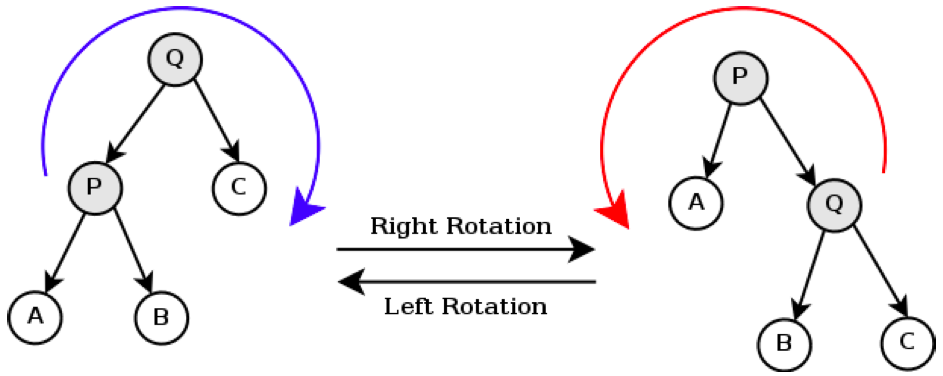
\includegraphics[width = 6cm]{avl.png}

AVL trees are \textbf{augmented} with height. \\
Trees can be augments with size of node's subtree to make rank a search while accumulating the tag.

\subsubsection{Notation}
\begin{itemize}
\item$d[v]$ is length of current shortest path from $s$ to $v$ (evolves over search) 
\item$\pi [v]$ is current parent of $v$ 
\item$\delta (s,v)$ is length of actual shortest path from $s$ to $v$
\end{itemize}

\subsection{Breadth-First Search}
\textbf{Invariant:} When adding a node $v$ into the BFS tree induced by $s$, where $v$ is $k$ edges away from $s$, all nodes currently in the BFS tree are $\le k$ edges away from $s$.
\begin{itemize}
	\item Queue 
	\item Unweighted digraph
	\item Guarantees shortest path 
	\item $\Theta(|V| + |E|)$
\end{itemize}

\subsection{Depth-First Search}
\begin{itemize}
	\item Stack 
	\item Reverse finish order is topological sort
	\item Guarantees shortest path 
	\item $\Theta(|V| + |E|)$
\end{itemize}

\subsection{Topological Sort}
Topological ordering of a graph $G$ is an ordering of its vertices $[v_0, v_1, , v_n]$ in such a way that all the edges point from left to right (all edges $(v_i,v_j)$ $\in$ $E$ such that $i <j$). A valid topo. \\
Ordering is obtained by reversing the order of recursive calls in a DFS traversal. ($O(V + E)$ time).

\subsection{Tree Edge Types}
\begin{itemize}
	\item \textbf{Tree Edge -} an edge along which a discovery was made.
	\item \textbf{Back Edge -} when looking down that edge you see a discovered ancestor node.
	\item \textbf{Forward Edge -} when looking down that edge you see a discovered descendant node.
	\item \textbf{Cross Edge -} when looking down that edge you see a discovered node that is not an ancestor or descendant. An edge which points from a node on a subtree to a node on a different subtree.
\end{itemize}
Undirected graphs have no forward edges or corss edges in their resulting search tree.

\subsection{Dijkstra}
Requires positive weights. Can have cycles, may not terminate with negative cycles. \\
An \textbf{unprocessed} node has not yet been removed from Q. It may have a finite $d[v]$. \\
Runtime: $\Theta(|V|\cdot$insert$+|V|\cdot$extraction$+|V|\cdot$decrease-key$)$
\\ = $\Theta(\log(|V|(|V|+|E|)))$ with a min-heap

\subsection{Bellman-Ford}
$|V|$ relaxations of $|E|$ edges: $O(|V| \cdot |E|)$ \\
Can be used to detect negative cycles (Negative cycle exists along path if no shortest path exists)

%---------------------------------------------------------------------------

\section{Numerics}

\subsection{Catalan Numbers}
How many ways to group $n$ factors with parenthesis. Call this number $P_n$.
\begin{align*}
C_n =& \frac{1}{n+1} \binom{2n}{n} \\
P_n =& \frac{1}{n}\binom{2(n-1)}{n-1} = \sum_{k=1}^{n-1}P_kP_{n-k} = C_{n-1}
\end{align*}
\subsection{Karatsuba}
Naive multiplication is $O(n^2)$. Karatsuba is $O(n^{\log_2 (3)})$. \\

If $x$ is $n$ bits, we can write it as $x_1 \cdot 2^{\frac{n}{2}} +x_0$ where $x_1$ and $x_0$ are the 2 halves of the bits in $x$.
\begin{align*}
z0 =& x0 \cdot y0 \\
z_1 =& x_1 \cdot y_1 \\
z_2 =& (x_0 +x_1)(y_0 +y_1)- (z_0 + z_1)  \\
z_2 =& x_0 \cdot y_1 +x_1 \cdot y_0 
\end{align*}

Recurrence: $T(n) = 3T( \frac{n}{2}) + \Theta(n) = \Theta(n^{\log_2(3)})$

\subsection{Newton's Method}
$x_{i+1} = x_i - f(x_i) / f'(x_i)$ where $f(x)$ is the function we are finding the root of \\
High precision division: $\frac{a}{b} = a \cdot \frac{1}{b}$. Use $f(x) = \frac{1}{x} - b$ \\
Runtime: Newton's method converges quadratically (double digits of precision each iteration) assuming a first guess within 1 of the correct answer. O(log(digits of precision))
%---------------------------------------------------------------------------
\section{Graph Theory}
\SetVertexNormal[Shape      = circle,
                 FillColor  = white,
                 LineWidth  = 2pt]
\SetUpEdge[lw         = 1.5pt,
           color      = black,
           labelcolor = white,
           labeltext  = black,
           labelstyle = {sloped,draw,text=blue}]
\begin{center}
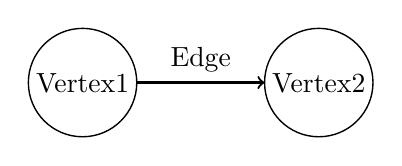
\begin{tikzpicture}
   \Vertex[x=0 ,y=0]{Vertex1}
   \Vertex[x=3 ,y=0]{Vertex2}
   \tikzset{EdgeStyle/.style={->}}
   \Edge[label={Edge}, labelstyle={above}](Vertex1)(Vertex2)
\end{tikzpicture}
\end{center}

\subsection{Simple Graphs}
Degree = $\#$ of incident edges \\
\textbf{Handshake Lemma:} $\Sigma deg(V) = 2|E|$, $v \in V$
\subsubsection{Connectivity}
Subgraphs of connected components. \\
K-connectivity: k-edge connected iff every 2 vertices are k-edge connected. \\
i.e. cycle is 2-connected, tree is 1-connected, complete is n-1-connected. \\

\subsection{Directed Acyclic Graphs}
Directed graph with no positive length cycles. \\
Vertex, $v$, of DAG, $D$, is minimum iff every other vertex is reachable from $v$. \\
\subsubsection{Antichain}
Set of vertices such that no 2 elements in the set are comparable.
\begin{itemize}
\item[\textbf{1)}] If largest chain is $t$, $V(0)$ can be partitioned into $t$ antichains.
\item[\textbf{2)}] (Dilworth) $\forall t > 0$, every DAG with $n$ vertices must have a chain size $> t$ or an antichain size $\ge \frac{n}{t}$.
\item[\textbf{3)}] Every DAG with $n$ vertices has a chain size $> \sqrt{n}$ or antichain size $\ge \sqrt{n}$.
\end{itemize}

\subsection{Adjacency list}
Adjacency list (list of edges, good for graphs with relatively few edges), or as a $V \times V$ matrix $G$. \\
Edge is defined if G[row][col] is defined.

%---------------------------------------------------------------------------
\section{Dynamic Programming}
$T$ $=$ ($\#$ subproblems) $\times$ (time per subproblem)

\subsection{Steps}
\begin{itemize}
\item[1] Define subproblems
\item[2] Guess (part of solution)
\item[3] Relate subproblem solutions
\item[4] Recurse + memoize
\item[ ] OR build DP table bottom-up
\item[ ]check subproblems acyclic/topological order
\item[5]Solve original problem: = a subproblem
\item[ ]OR by combining subproblem solutions
\end{itemize}
suffixes $x[i :]$ and prefixes $x[: i]$; $T$ = $\Theta(|x|)$ \\
substrings $x[i : j]$; $T$ = $\Theta(x^2)$

\subsection{Memoized Recursive}
Add a memo dictionary to store outputs for each input combination (subproblem) solved so far. \\
To solve a subproblem that's not in the memo, we just run our original recursive algorithm and then store the result in memo. \\
Often much easier to understand \\
Don't have to determine an ordering, which might be hard to do manually in some cases

\subsection{Bottom-up}
Rather than letting the recursive algorithm solve the subproblems on an on-demand basis, we can choose to build up our subproblems from the base cases up, in such a way that every time we solve a subproblem any subproblems it refers to are already solved. \\
Finding such an ordering is equivalent to topologically sorting the DAG defined by the dependencies of each subproblem. \\
Doesn't have the overhead of recursion (we also avoid the issue of exceeding the maximum recursion depth, due to extremely deep recursions) \\ 
Often easier to analyze runtime

%---------------------------------------------------------------------------
\section{Complexity}
\begin{tabular}{r | l}
P & Problems solvable in \textbf{polynomial}, $n^c$ time \\
NP & Decision problems whose solutions can be verified in \textbf{polynomial} time \\
EXP & Problems solvable in \textbf{exponential}, $2^{n^c}$ time \\
R & Problems solvable in \textbf{finite} time \\
\end{tabular}
\\
\textbf{Important relationship:} P $\subset$ EXP $\subset$ R \\
\textbf{Important relationship:} P $\subseteq$ NP \\
\textbf{Important open-problem:} P $\neq$ NP, believed to be true \\
\ \\
NP-hard: problems that are as hard as any problem in NP. \\
NP-complete: problems that are in NP and are NP-hard. \\
EXP-hard: problems that are as hard as any problem in EXP. \\ 
EXP-complete: problems that are in EXP and are EXP-hard. 

\subsection{Reduction}
Transforming an input for A into an input for B. \\
Any problem B that you can reduce A to will have to be at least as hard as A.\\
\subsubsection{Example NP hard problems}
\begin{itemize}
\item Longest simple path in a graph
\item Hamiltonian path
\item Hamiltonian cycle
\end{itemize}

%---------------------------------------------------------------------------
\section{Proof}

To prove an algorithm, demonstrate:
\begin{itemize}
\item Termination (it does not go on forever)
\item safety (the result it produces is always correct).
\end{itemize}

If the proof is non-trivial, use one of the following proof techniques to construct a well-argued proof (proof by example, or proof by long paragraph of rambling text are not proofs):
\begin{itemize}
\item \textbf{Contradiction}: Assume the thing you are proving is false, and show that it leads to obviously false conclusions. This is usually the way to go. Example: prove there is no largest integer. Suppose that this is false, and there exists some largest integer $k$. But $k + 1 > k$ is also an integer, so $k$ cannot be largest. But k is defined as the largest integer! Therefore the initial statement must be false, and there is no largest integer.
\item \textbf{Induction}: In the case of a recursive algorithm, prove the base case (when it does not make a recursive call), then prove the inductive case (often by contradiction, by assuming the recursive call does the right thing and extending this to show the entire algorithm does the right thing).
\end{itemize}

%---------------------------------------------------------------------------
\section{When to Use Tricks}
\subsection{Data Structures}
\begin{tabular}{r | l}
Need & Algorithm  \\ \hline
If no cleverness needed & Unordered array \\
If all data upfront & Sorted array \\
If seen “min” or “max” & Binary Min/Max Heap  \\
If need to store sorted dynamic data & BST with AVL \\
If unordered data & Dictionary \\
\end{tabular}

\subsection{Shortest Path}
\begin{tabular}{r | c | l}
Need & Algorithm & Runtime \\ \hline
Unweighted graphs & BFS & $O(|E|)$ \\
Weighted DAGs & Topological Sort & $O(V+E)$ \\
Weighted graphs w/o $\neg E$ & Dijkstra & $\Theta(\log(|V|(|V|+|E|)))^\ast$ \\
Non-DAG w/ $\neg E$ & Bellman Ford & $O(|V| \cdot |E|)$\\
\end{tabular}
$\ast$ With a min-heap \\

\subsection{Other}
\textbf{Single-source shortest-paths problem:} \\
Find a shortest path from a source vertex to each other vertex in the graph (Bellman-Ford, Dijkstra) \\
\textbf{Single-destination shortest-paths problem:} \\
Find a shortest path to a destination vertex from each other vertex in the graph (Bellman-Ford/Dijkstra on reversed graph) \\
\textbf{Single-pair shortest-path problem:} \\
Find a shortest path between a vertex u and a vertex v in a graph (Bellman-Ford, Dijkstra)\\
\textbf{All-pairs shortest-paths problem:} \\
Find a shortest path between every two vertices in a graph (Bellman-Ford/Dijkstra V times, Floyd-Warshall) \\

\textbf{If vague template for all shortest path algorithms,repeat until done:} \\
Pick edge u to v element E: relax v.d using (u to v) \\
Relax compares the “previous best” distance v.d with newfound path u.d + weight(u to v), and updates the path if it is indeed shorter. \\
This takes $O(1)$ time.\\

\textbf{Shortest path with even or odd length:} \\
Make a new graph $G'$. For every vertex $u$ in $G$, there are two vertices $u_E$ and $u_O$ in $G'$: these represent reaching the vertex u through even and odd number of edges respectively. For every edge $(u, v)$ in $G$, there are two edges in $G'$: $(u_E, v_O)$ and ($u_E$; $v_E$). Both of these edges have the same weight as the original. \\
Runs in linear time $O(V + E$). Then we can run shortest path algorithms from $s_E$ to $t_O$.

\textbf{If Longest path:} \\
Longest path on DAG = Shortest path on DAG with edge weights multiplied by (-1)

%---------------------------------------------------------------------------
\section{Pseudo-code}
\begin{alltt}

TOPOLOGICAL-SORT(G): 
\ \	dfs_result = DFS(G) 
\ \	dfs_result.order.reverse() 
\ \	return dfs_result.order

RELAX(u,v,w)
\ \	if v.d > u.d + w(u,v)
\ \	\ \	v.d = u.d + w(u,v)
\ \	\ \	v.\(\pi\) = u

DAG-SHORTEST-PATHS(G,w,s)
\ \	topologically sort the vertices of G
\ \	INITIALIZE-SINGLE-SOURCE(G,s)
\ \	for each vertex u, taken in topologically sorted order 
\ \	\ \	for each vertex v \(\in\) G:Adj[]
\ \	\ \	\ \	RELAX(u,v,w)

DIJKSTRA(G,w,s)
\ \	INITIALIZE-SINGLE-SOURCE(G,s)
\ \	S = 0	
\ \	Q = G.V 
\ \	while Q \(\neq\) 0: 
\ \	\ \	u = EXTRACT-MIN(Q) 
\ \	\ \	S = S fug 
\ \	\ \	for each vertex v \(\in\) G:Adj[]
\ \	\ \	\ \	RELAX(u,v,w)

BELLMAN-FORD(G,w,s)
\ \	INITIALIZE-SINGLE-SOURCE(G,s)
\ \	for i=1 to |G:V| - 1
\ \	\ \	for each edge (u,v) \(\in\) G.E
\ \	\ \	\ \	RELAX(u,v,w)
\ \	for each edge (u,v) \(\in\) G.E
\ \	\ \	if v.d > u.d + w(u,v)
\ \	\ \	\ \	return FALSE
\ \	return TRUE

DAG-Bellman-Ford(V, E, s) 
\ \	TopologicallySort(V, E) 
\ \	Initialize(V, E) 
\ \	for each vertex u \(\in\) V taken in topological order 
\ \	\ \	for each edge originating at u, (u, v) \(\in\) E
\ \	\ \	\ \	Relax(u, v)

memo = dictionary
MEM-RECURSE-FIB(n): 
\ \	if n in memo: 
\ \	\ \	return memo[n] 
\ \	else: if n \(\le\) 2 : f = 1 
\ \	\ \	else: f = fib(n-1)+fib(n-2) 
\ \	\ \	memo[n] = f 
\ \	\ \	return f

BOTTOM-UP-FIB(n):
\ \	fib = dictionary 
\ \	for k in [1, 2, . . . , n]: 
\ \	\ \	if k \(\le\) 2: f = 1 
\ \	\ \	else: f = fib[k-1] + fib[k-2]
\ \	\ \	fib[k] = f
\ \	return fib[n]
\end{alltt}

%---------------------------------------------------------------------------
\section{Examples}
\subsection{Change of Variables}
\begin{align*}
T(n) =& \ 2T(\sqrt{n}) + \Theta(\log(n)), \ \ \ \ \ \ \ \ \ n = 2^m \\
T(2^m) =& \ 2T(\sqrt{2^m}) + \Theta(log(2^m)) \ = \ 2T(2^{\frac{m}{2}})) + \Theta(m) \\
S(m) =& \ T(2^m) = T(n) \\
S(m) =& \ 2S(\frac{m}{2}) + \Theta(m) \\
S(m) =& \ \Theta(m \log(m)) \\
T(n) =& \ \Theta(\log(n)\log(\log(n))) \\
\end{align*}

\subsection{Newton Reciprocal}
Find reciprocal $b^{-1}$
\begin{itemize}
\item[Root:] $f(x) = \frac{1}{x} - b$
\item[ ] $f'(x) = \frac{-1}{x^2}$
\item[Newton:] $x_{i+1} := x_i - \frac{\frac{1}{x_i}-b}{\frac{-1}{x^2}}$ 
\item[ ] $x_{i+1} := 2x_i - bx_i^2$
\end{itemize}

\subsection{The Knapsack Problem}
$dp[i][j]$ is the maximum value that can be obtained by using a subset of the items $i ...n-1$ (last $n-i$ items) which weighs at most $j$ pounds. When computing $dp[i][j]$, we need to consider all the possible values of $d_i$ (the decision at step $i$) \\
\begin{alltt}
KNAPSACK(n, S, s, v) 
\ \	for i in [n,n-1...0]
\ \	\ \	for j in [0, 1 . . . S]
\ \	\ \	\ \	if i == n: dp[i][j] = 0 \(\rhd\) initial condition 
\ \	\ \	\ \	else:
\ \	\ \	\ \	\ \	choices = [] 
\ \	\ \	\ \	\ \	APPEND(choices, dp[i + 1][j]) 
\ \	\ \	\ \	\ \	if j \(\ge\) si: APPEND(choices, dp[i + 1][j - si] + vi) 
\ \	\ \	\ \	\ \	dp[i][j] = MAX(choices) 
return dp[0][S]
\end{alltt}
The dynamic programming solution to the Knapsack problem requires solving $O(nS)$ sub-problems. The solution running time is \textbf{not polynomial} in the input size, instead this algorithm is said to run in \textbf{pseudo-polynomial} time.

\rule{0.3\linewidth}{0.25pt}
\scriptsize

“Experience is simply the name we give our mistakes.” \\
 $-$ Oscar Wilde



\end{multicols}
\end{document}